\documentclass[border=2pt]{standalone}
% Shared TikZ style contract for every schematic figure in this paper.
% Each schematic is a standalone document that \input's this file, so the
% schematics and the matplotlib data figures form one visual system.
%
% Colours are the same Okabe-Ito values as figures/scifig_style.py.

% No font package: the manuscript class sets the body in Computer Modern, so
% the schematics inherit the same family by loading nothing here.
\usepackage{amsmath,amssymb}
\usepackage{tikz}
\usetikzlibrary{arrows.meta,positioning,calc,fit,backgrounds,shapes.geometric,
                shapes.multipart,patterns,decorations.pathreplacing,matrix}

% ---------- Notation shared with the manuscript ----------
% Kept in sync with the definitions in main.tex so that a symbol means the
% same thing in a schematic as it does in the body.
\newcommand{\Cmax}{C_{\max}}
\newcommand{\Zcost}{Z}
\newcommand{\Nb}{\mathcal{N}}

% ---------- Okabe-Ito colour-blind-safe palette ----------
\definecolor{oiblue}{RGB}{0,114,178}
\definecolor{oiorange}{RGB}{230,159,0}
\definecolor{oigreen}{RGB}{0,158,115}
\definecolor{oivermilion}{RGB}{213,94,0}
\definecolor{oipurple}{RGB}{204,121,167}
\definecolor{oisky}{RGB}{86,180,233}
\definecolor{oiyellow}{RGB}{240,228,66}
\definecolor{oigray}{RGB}{110,110,110}

% ---------- Shared node and arrow styles ----------
\tikzset{
  block/.style={draw, rounded corners=2pt, minimum height=6.5mm, minimum width=17mm,
                align=center, font=\footnotesize, fill=oisky!16, line width=0.6pt,
                draw=oiblue!70},
  keyblock/.style={block, fill=oiorange!26, draw=oiorange!85},
  smallblock/.style={block, minimum height=5mm, minimum width=12mm, font=\scriptsize},
  datanode/.style={draw, trapezium, trapezium left angle=70, trapezium right angle=110,
                   align=center, font=\scriptsize, fill=oigreen!14, line width=0.6pt,
                   draw=oigreen!75, inner sep=2pt},
  opnode/.style={draw, circle, inner sep=1pt, minimum size=6mm, font=\scriptsize,
                 fill=oiyellow!45, line width=0.6pt, draw=oigray},
  macnode/.style={draw, rectangle, rounded corners=1pt, minimum size=6mm,
                  font=\scriptsize, fill=oisky!30, line width=0.6pt, draw=oiblue!70},
  modnode/.style={draw, diamond, aspect=1.4, inner sep=1pt, minimum size=6mm,
                  font=\scriptsize, fill=oipurple!28, line width=0.6pt, draw=oipurple!85},
  arrow/.style={-{Stealth[length=2.0mm]}, line width=0.65pt},
  dasharrow/.style={arrow, dashed, draw=oigray},
  thinedge/.style={line width=0.45pt, draw=oigray},
  note/.style={font=\scriptsize, text=oigray, align=center},
  tinynote/.style={font=\tiny, text=oigray, align=center},
  group/.style={draw=oigray, dashed, rounded corners=3pt, inner sep=2.6mm,
                line width=0.5pt},
  grouplabel/.style={font=\scriptsize\itshape, text=oigray},
  whitebg/.style={fill=white, inner sep=1pt},
}

\begin{document}
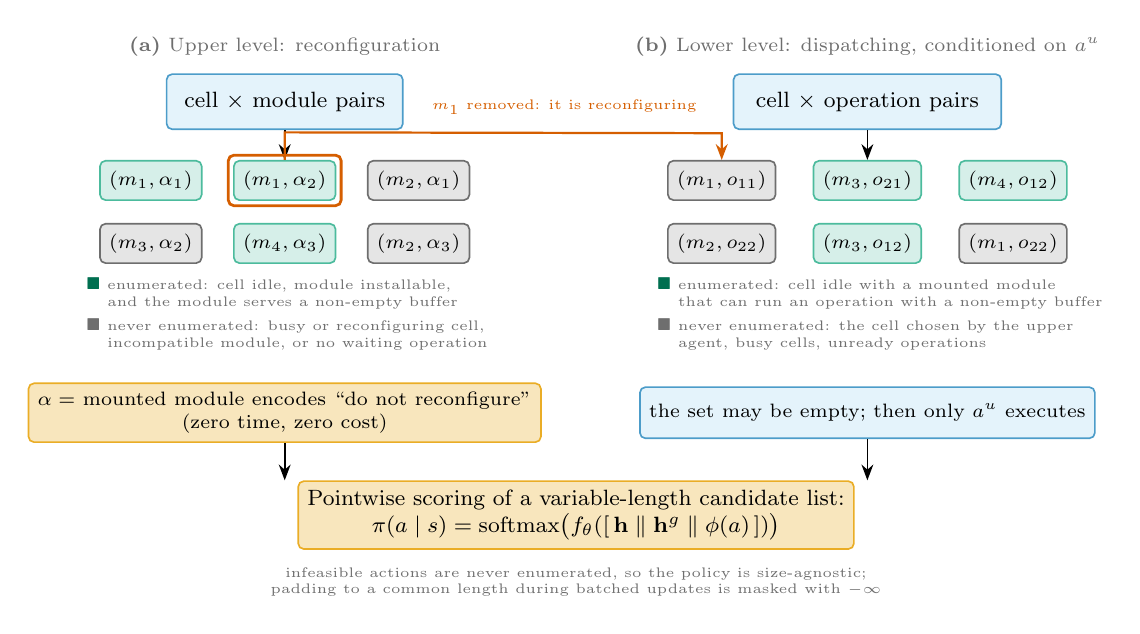
\begin{tikzpicture}

% ================= (a) upper level =================
\node[note] at (0,3.05) {\textbf{(a)} Upper level: reconfiguration};
\node[block, minimum width=30mm, minimum height=7mm] (ustate) at (0,2.35)
  {cell $\times$ module pairs};

\node[smallblock, fill=oigreen!16, draw=oigreen!70] (u1) at (-1.7,1.35) {$(m_1,\alpha_1)$};
\node[smallblock, fill=oigreen!16, draw=oigreen!70] (u2) at (0.0,1.35) {$(m_1,\alpha_2)$};
\node[smallblock, fill=oigray!18, draw=oigray] (u3) at (1.7,1.35) {$(m_2,\alpha_1)$};
\node[smallblock, fill=oigray!18, draw=oigray] (u4) at (-1.7,0.55) {$(m_3,\alpha_2)$};
\node[smallblock, fill=oigreen!16, draw=oigreen!70] (u5) at (0.0,0.55) {$(m_4,\alpha_3)$};
\node[smallblock, fill=oigray!18, draw=oigray] (u6) at (1.7,0.55) {$(m_2,\alpha_3)$};

\node[tinynote, align=left, anchor=west] at (-2.65,-0.35)
  {\textcolor{oigreen!70!black}{$\blacksquare$} enumerated: cell idle, module installable,\\
   \phantom{$\blacksquare$} and the module serves a non-empty buffer\\[1mm]
   \textcolor{oigray}{$\blacksquare$} never enumerated: busy or reconfiguring cell,\\
   \phantom{$\blacksquare$} incompatible module, or no waiting operation};

\node[keyblock, minimum width=32mm, font=\scriptsize] (unote) at (0,-1.6)
  {$\alpha=$ mounted module encodes ``do not reconfigure''\\(zero time, zero cost)};

\draw[arrow] (ustate) -- (u2);
\node[draw=oivermilion, line width=1.0pt, rounded corners=2pt, fit=(u2), inner sep=0.6mm] {};

% ================= (b) lower level =================
\node[note] at (7.4,3.05) {\textbf{(b)} Lower level: dispatching, conditioned on $a^{u}$};
\node[block, minimum width=34mm, minimum height=7mm] (lstate) at (7.4,2.35)
  {cell $\times$ operation pairs};

\node[smallblock, fill=oigray!18, draw=oigray] (l1) at (5.55,1.35) {$(m_1,o_{11})$};
\node[smallblock, fill=oigreen!16, draw=oigreen!70] (l2) at (7.4,1.35) {$(m_3,o_{21})$};
\node[smallblock, fill=oigreen!16, draw=oigreen!70] (l3) at (9.25,1.35) {$(m_4,o_{12})$};
\node[smallblock, fill=oigray!18, draw=oigray] (l4) at (5.55,0.55) {$(m_2,o_{22})$};
\node[smallblock, fill=oigreen!16, draw=oigreen!70] (l5) at (7.4,0.55) {$(m_3,o_{12})$};
\node[smallblock, fill=oigray!18, draw=oigray] (l6) at (9.25,0.55) {$(m_1,o_{22})$};

\draw[arrow] (lstate) -- (l2);
% conditioning arrow routed through the free corridor between the two panels
\draw[arrow, draw=oivermilion, line width=0.8pt]
  (u2.north) -- ++(0,0.35) -- (5.55,1.95) -- (l1.north);
\node[tinynote, text=oivermilion, align=center] at (3.55,2.28)
  {$m_1$ removed: it is reconfiguring};

\node[tinynote, align=left, anchor=west] at (4.6,-0.35)
  {\textcolor{oigreen!70!black}{$\blacksquare$} enumerated: cell idle with a mounted module\\
   \phantom{$\blacksquare$} that can run an operation with a non-empty buffer\\[1mm]
   \textcolor{oigray}{$\blacksquare$} never enumerated: the cell chosen by the upper\\
   \phantom{$\blacksquare$} agent, busy cells, unready operations};

\node[block, minimum width=32mm, font=\scriptsize] (lnote) at (7.4,-1.6)
  {the set may be empty; then only $a^{u}$ executes};

% ================= (c) scoring =================
\node[keyblock, minimum width=46mm, minimum height=8mm] (score) at (3.7,-2.9)
  {Pointwise scoring of a variable-length candidate list:\\
   $\pi(a\mid s)=\mathrm{softmax}\big(f_\theta([\,\mathbf{h}\;\|\;\mathbf{h}^{g}\;\|\;\phi(a)\,])\big)$};
\draw[arrow] (unote) -- (unote |- score.north);
\draw[arrow] (lnote) -- (lnote |- score.north);
\node[tinynote, align=center] at (3.7,-3.75)
  {infeasible actions are never enumerated, so the policy is size-agnostic;\\
   padding to a common length during batched updates is masked with $-\infty$};

\end{tikzpicture}
\end{document}
